% $Header: /Users/joseph/Documents/LaTeX/beamer/solutions/conference-talks/conference-ornate-20min.en.tex,v 90e850259b8b 2007/01/28 20:48:30 tantau $

\documentclass{beamer}

\usepackage[font={footnotesize}]{caption}
\usepackage[
	backend=biber,
	style=authortitle,
	doi=false,
	% isbn=false, 
	maxcitenames=2,
]{biblatex}
\addbibresource{master.bib}

\definecolor{viridis_01}{rgb}{0.267004, 0.048740, 0.329415}
\definecolor{viridis_02}{rgb}{0.190631, 0.407061, 0.556089}
\definecolor{viridis_03}{rgb}{0.208030, 0.718701, 0.472873}
\definecolor{viridis_04}{rgb}{0.993248, 0.906157, 0.143936}

% \AtEveryCite{\color{viridis_03}}

% This file is a solution template for:

% - Talk at a conference/colloquium.
% - Talk length is about 20min.
% - Style is ornate.

% Copyright 2004 by Till Tantau <tantau@users.sourceforge.net>.
%
% In principle, this file can be redistributed and/or modified under
% the terms of the GNU Public License, version 2.
%
% However, this file is supposed to be a template to be modified
% for your own needs. For this reason, if you use this file as a
% template and not specifically distribute it as part of a another
% package/program, I grant the extra permission to freely copy and
% modify this file as you see fit and even to delete this copyright
% notice. 

\mode<presentation>
{
  % \usetheme{default}
  % \usecolortheme{beaver}
  \setbeamercolor{structure}{fg=viridis_01,bg=black!10!}
  % \setbeamercolor{palette secondary}{fg=viridis_02}

}


\usepackage[english]{babel}
% or whatever

\usepackage[latin1]{inputenc}
% or whatever

% \usepackage{times}
\usepackage[T1]{fontenc}
\usepackage{graphics}
\usepackage{caption}
\usepackage{siunitx}
% Or whatever. Note that the encoding and the font should match. If T1
% does not look nice, try deleting the line with the fontenc.

\beamertemplatenavigationsymbolsempty
\usefonttheme{serif}

\title[Short title] % (optional, use only with long paper titles)
{Title}

% \subtitle
% {
% }

\author % (optional, use only with lots of authors)
{Daniel M. Bj\o rnstad}
% - Give the names in the same order as the appear in the paper.
% - Use the \inst{?} command only if the authors have different
%   affiliation.

\date{April 26, 2016}

\institute
{
    CINPLA - Weekly Meeting
}




% If you have a file called "university-logo-filename.xxx", where xxx
% is a graphic format that can be processed by latex or pdflatex,
% resp., then you can add a logo as follows:

% \pgfdeclareimage[height=0.5cm]{university-logo}{university-logo-filename}
% \logo{\pgfuseimage{university-logo}}



% Delete this, if you do not want the table of contents to pop up at
% the beginning of each subsection:
%
%\AtBeginSubsection[]
%{
  %\begin{frame}<beamer>{Outline}
  %  \tableofcontents[currentsection,currentsubsection]
  %\end{frame}
%}


% If you wish to uncover everything in a step-wise fashion, uncomment
% the following command: 

%\beamerdefaultoverlayspecification{<+->}


\begin{document}

\begin{frame}
  \titlepage
\end{frame}

%\begin{frame}{Outline}
%  \tableofcontents
  % You might wish to add the option [pausesections]
%\end{frame}


% Structuring a talk is a difficult task and the following structure
% may not be suitable. Here are some rules that apply for this
% solution: 

% - Exactly two or three sections (other than the summary).
% - At *most* three subsections per section.
% - Talk about 30s to 2min per frame. So there should be between about
%   15 and 30 frames, all told.

% - A conference audience is likely to know very little of what you
%   are going to talk about. So *simplify*!
% - In a 20min talk, getting the main ideas across is hard
%   enough. Leave out details, even if it means being less precise than
%   you think necessary.
% - If you omit details that are vital to the proof/implementation,
%   just say so once. Everybody will be happy with that.

\begin{frame}{Introduction}
    L5 P14 male Wistar Han rats. Seperated into morphological and 
    electrophysiological types
\end{frame}

\begin{frame}{Introduction}
    \begin{figure}
        \centering
        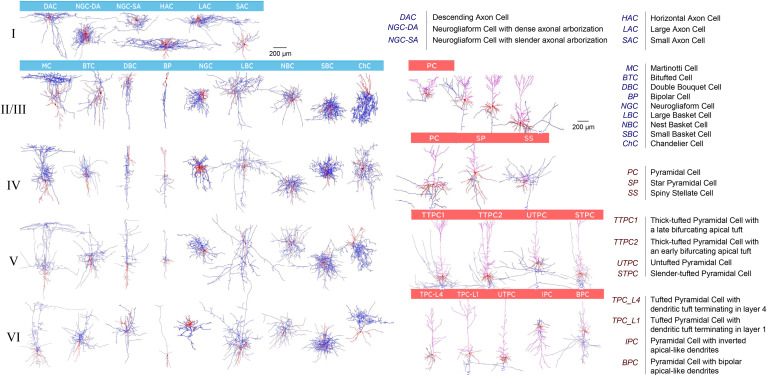
\includegraphics[width=\textwidth]{images/m-types.jpg}\\
        \caption*{\centering Fig. 2 in \textcite{markram_reconstruction_2015}}
    \end{figure}
\end{frame}

\begin{frame}{Introduction}
    \begin{figure}
        \centering
        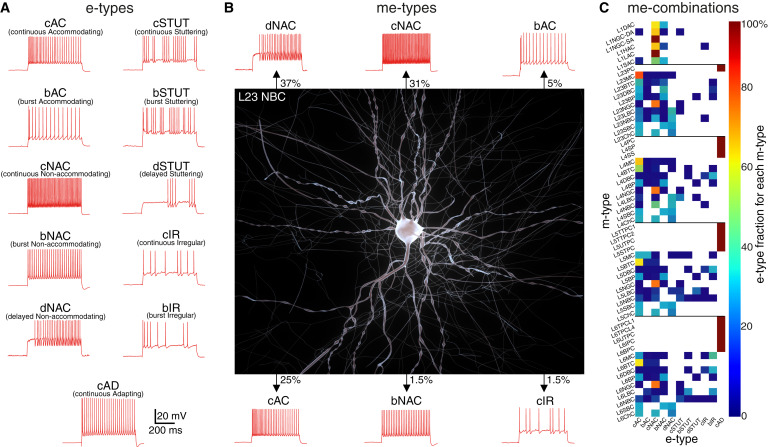
\includegraphics[width=\textwidth]{images/e-types.jpg}\\
        \caption*{\centering Fig. 4 in \textcite{markram_reconstruction_2015}}
    \end{figure}
\end{frame}

\begin{frame}{Optimal Width Definition}{}
\end{frame}

\begin{frame}{Optimal Amplitude Definition}
\end{frame}

\begin{frame}{Combine Width and Amplitude}
\end{frame}

\begin{frame}{Other Spike Width Results}
\end{frame}



\end{document}
